\chapter{Kotlin}                %crea il capitolo
%%%%%%%%%%%%%%%%%%%%%%%%%%%%%%%%%%%%%%%%%imposta l'intestazione di pagina
\lhead[\fancyplain{}{\bfseries\thepage}]{\fancyplain{}{\bfseries\rightmark}}
\pagenumbering{arabic}                  %mette i numeri arabi
\section{Storia}                 %crea la sezione

Kotlin è un linguaggio di programmazione open source\footnote{https://github.com/JetBrains/kotlin}, basato sulla JVM (Java Virtual Machine), con la caratteristica di essere orientato agli oggetti e staticamente tipizzato. \\
Lo sviluppo di Kotlin è iniziato nel 2010 dall'azienda JetBrains, conosciuta nel modo dello sviluppo software Java per la realizzazione di diversi IDE (Integrated development environment), tra cui: Intellij IDEA, sul quale si basa l'attuale IDE di Google dedicato alla programmazione Android, chiamato: Android Studio.\\
Il team di JetBrains, scelse di iniziare a realizzare un nuovo linguaggio di programmazione, per risolvere problematiche riscontrate durante la realizzazione dei loro IDE, in particolare Dmitry Jemerov, un programmatore di JetBrains e sviluppatore di Kotlin, rivelò durante un'intervista\footnote{https://www.infoworld.com/article/2622405/java/jetbrains-readies-jvm-based-language.html} che non esisteva ancora nessun linguaggio con le potenzialità e facilità d'uso richieste dal team di JetBrains, ad eccezione del linguaggio Scala che offriva grossi vantaggi nello sviluppo, ma aveva un tempo di compilazione molto lento, JetBrains scelse quindi di realizzare il linguaggio Kotlin basandosi sulla JVM, in seguito nel 2012 il progetto Kotlin venne resto Open Source sotto licenza ``Apache 2 license''.\\
Java fin dalle sue prime versioni, è sempre stato uno dei linguaggi  più usati e conosciuti ma presenta diverse imperfezioni e problemi che spinse il team di JetBrains a iniziare lo sviluppo di un suo linguaggio, con una sintassi semplice che prendesse in considerazione alcuni spunti e idee introdotte da linguaggi come CSharp, Scala, Groovy, ECMAScript, Go, Python, ma continuasse a basarsi sulla JVM.\\
L'idea di utilizzare pattern e idee di linguaggi preesistenti permise agli sviluppatori di introdurre la facilità sintattica, potenzialità e caratteristiche testate a lungo da altri linguaggi, senza dover apportare grosse innovazioni, rendendo quindi il linguaggio leggibile e comprensibile anche da chi non lo conoscesse.\\
Lo sviluppo di Kotlin si basava principalmente sul miglioramento di Java, ma dato che anche Android utilizzava la JVM, gli sviluppatori cercarono di adattarlo e renderlo ottimizzato anche per Android, come Java.\\
La comunità di sviluppatori che cominciò a utilizzare Kotlin crebbe enormemente, tra il 2016 e il 2017, in solo un anno, le linee di codice scritte in Kotlin su progetti presenti su GitHub quadruplicarono passando da 2.4 milioni a 10 milioni\footnote{https://blog.jetbrains.com/kotlin/2017/03/kotlin-1-1/} \\

\begin{figure}[!hb]
  \centering
  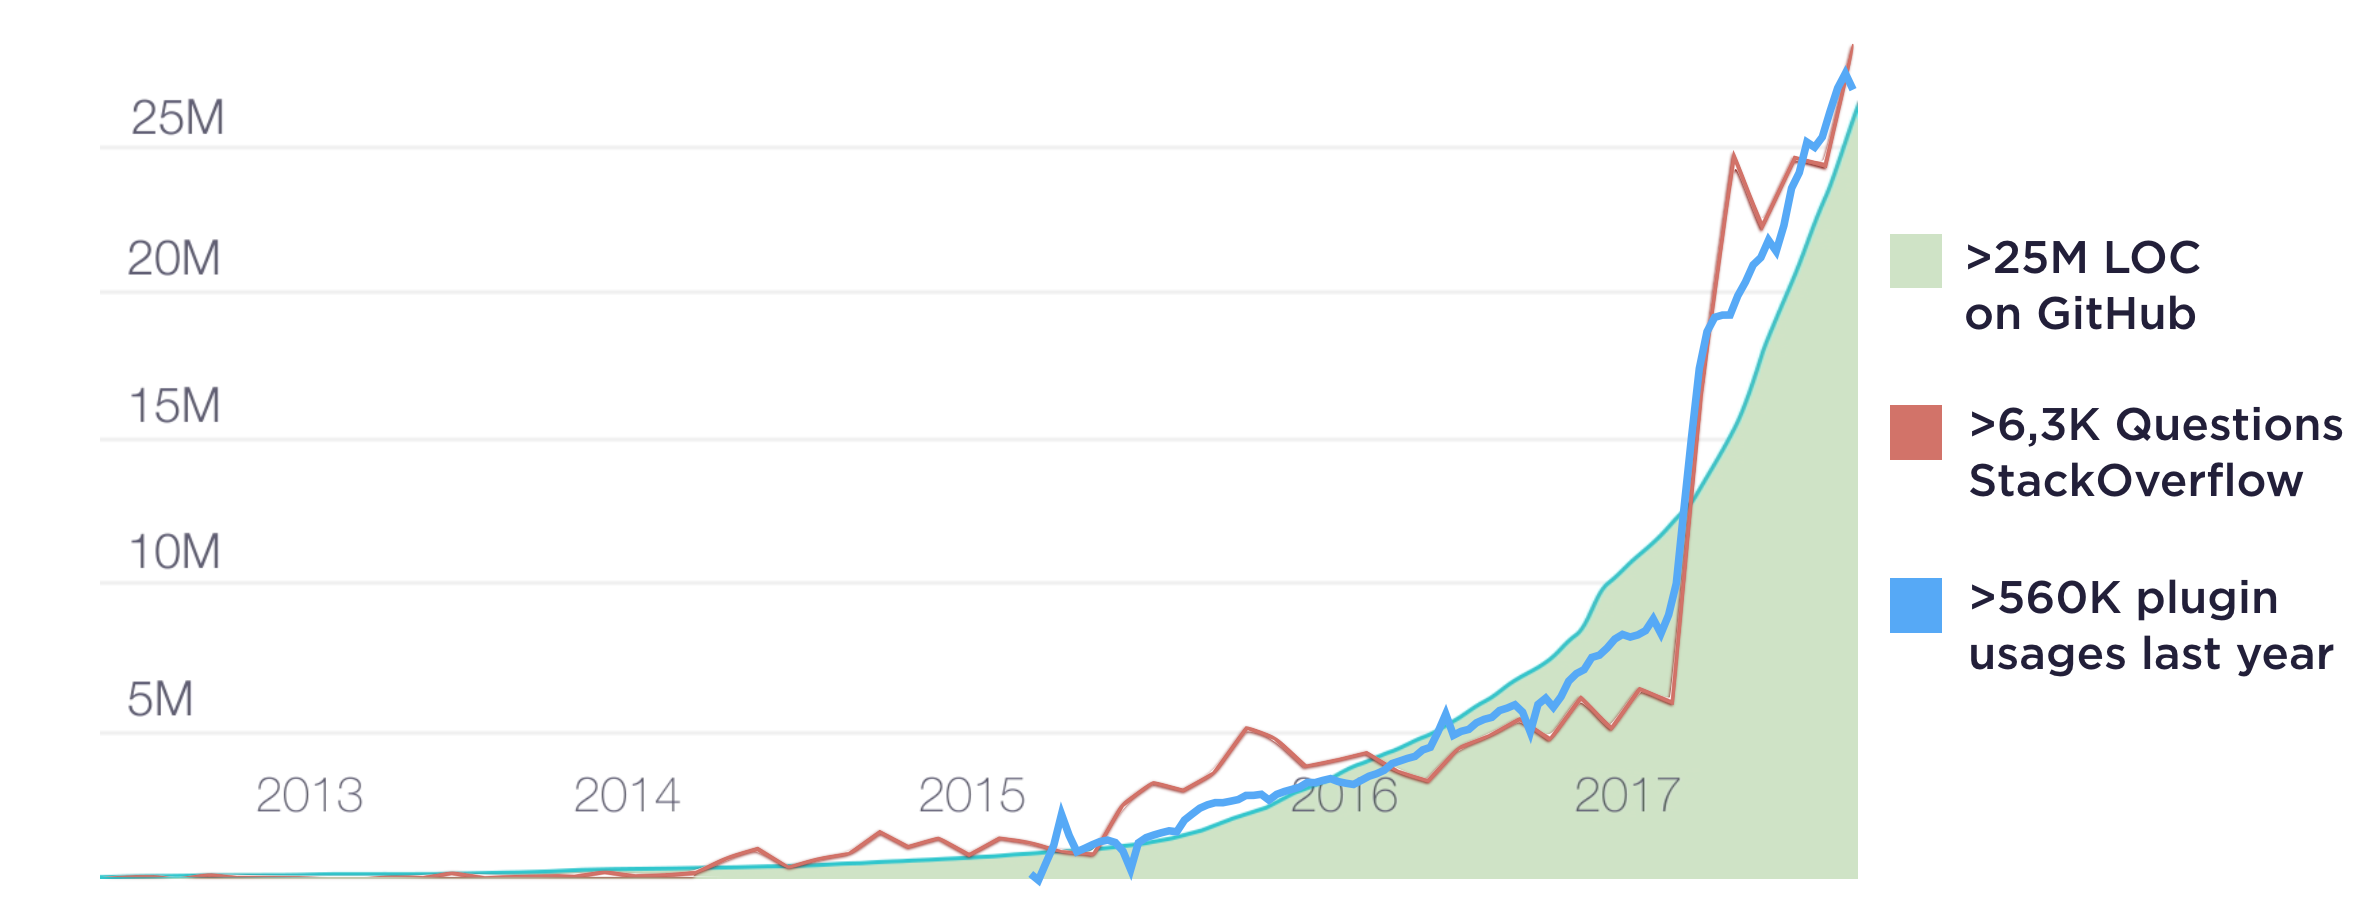
\includegraphics[width=0.85\textwidth]{immagini/kotlin_grafico_incremento.png}
  \caption{Grafico delle linee di codice scritte in Kotlin su Github.}\label{fig:Grafico delle linee di codice scritte in Kotlin su Github}
\end{figure}

Nel 2015 Google prese in considerazione l'utilizzo di Kotlin come plugin per Android Studio, e dopo vari test nel 2017 durante la conferenza Google IO 2017, arrivò l'annuncio che ufficializzava\footnote{https://android-developers.googleblog.com/2017/05/android-announces-support-for-kotlin.html} Kotlin come nuovo linguaggio di programmazione per lo sviluppo di applicazioni Android, senza escludere e rinunciare a Java, su cui si basa l'SDK di Android.\\
Gli stessi sviluppatori Android, dopo aver testato le potenzialità di Kotlin ne rimasero molto soddisfatti per la praticità, la stabilità ed i suoi benefici sintattici e funzionali, Kotlin è infatti un linguaggio molto coinciso, espressivo, strutturato sulla tipizzazione che mette a disposizione costrutti per evitare errori a puntatori nulli.\\
Il supporto completo di Kotlin su Android venne garantito attraverso una buona integrazione con Android Studio 3.0 e un plugin Kotlin per le versioni precedenti delle IDE, qualsiasi progetto che utilizzava Java poteva essere parzialmente o completamente convertito in Kotlin.





\section{Caratteristiche}
Il linguaggio Kotlin è stato sviluppato in ambito aziendale e non accademico, come spesso accade per altri linguaggi, rimanendo in fase beta per 7 anni, periodo in cui gli stessi programmatori che lavoravano presso JetBrains ne testarono le funzionalità, fino a raggiungere nel 2017 la prima versione stabile: la 1.0. \\
Kotlin è nato quindi all'interno di un team di sviluppatori che dopo anni di esperienza acquisita con Java e altri linguaggi hanno realizzato un linguaggio mirato a risolvere problematiche concrete riscontrati dagli stessi sviluppatori.\\
Prendendo spunto dalle problematiche di Java e da buone regole introdotte da alcuni linguaggi imperativi e funzionali, Kotlin è stato modellato in modo tale da aggiungere funzionalità utili sia a livello sintattico che a livello prestazionale, offrendo quindi al programmatore strumenti, caratteristiche e implementazioni semplici e utili ma molto potenti.\\
Un altro aspetto importante su cui il team di JetBrains ha prestato molta attenzione è stata la buona integrazione del suo plugin con Android Studio. Il supporto dato dal plugin è tale da supportare il programmatore in ogni momento, proponendo la riscrittura di porzioni di codice per renderlo più coinciso, allertare il programmatore in caso di possibili puntatori nulli, offrire una conversione automatica del codice Java in Kotlin e ove possibile cercare di avvisare lo sviluppatore su possibili problemi di prestazione ed errori sintattici.\\
Le caratteristiche più importanti offerte da Kotlin sono l'interoperabilità con Java, permettendo l'utilizzo di librerie Java e Kotlin simultaneamente, l'introduzione di alcune caratteristiche dei linguaggi di ordine superiore, la tipizzazione statica delle variabili, l'inferenza di tipo e soprattutto il null-safety consentendo di differenziare il tipo nullabile e il tipo non-nullabile, prevenendo quindi errori di "NullPointerExpetions".\\
Il codice prodotto in Kotlin \`e inoltre più compatto, coinciso e meno verboso grazie alle dataclass, il supporto delle lambda function e altri costrutti utili.


\subsection{Interoperabilità}
I linguaggi Kotlin e Java sono fortemente intercompatibili, permettendo quindi a entrambi i linguaggi di coesistere all'interno dello stesso progetto e di richiamare funzioni e parti di codice in Java da Kotlin e viceversa, poiché entrambi i linguaggi producono Java Bytecode\footnote{http://kotlinlang.org/docs/reference/java-interop.html}.\\
Prendiamo in considerazione il classico esempio ``Hello word'' scritto in Kotlin e in Java:

\begin{lstlisting}[language=java,caption={Hello World in Kotlin}]
fun main(args : Array<String>) {
  println("Hello, world!")
}
\end{lstlisting}

\begin{lstlisting}[language=java,caption={Hello World in Java}]
public class Hello {
    public static void main(String[] args) {
        System.out.println("Hello, world!");
    }
}
\end{lstlisting}

Il compilatore di Kotlin prendendo come input il file ``Hello.kt'' produrrà un JAR eseguibile da Java ``Hello.jar''

\begin{lstlisting}[language=bash,caption={Compilazione di un programma Kotlin}]
kotlinc Hello.kt -include-runtime -d Hello.jar
java -jar Hello.jar
Hello, world!
\end{lstlisting}

\'E possibile chiamare classi Java all'interno di funzioni Kotlin e viceversa:
\begin{lstlisting}[language=Kotlin,caption={Chiamare Java da Kotlin}]
 class KotlinClass {
     fun kotlinDoSomething() {
         val javaClass = JavaClass()
         javaClass.javaDoSomething()
         println(JavaClass().prop)
     }
 }
 \end{lstlisting}

 \begin{lstlisting}[language=java,caption={Chiamare Kotlin da Java}]
 public class JavaClass {
     public String getProp() { return "Hello"; }
     public void javaDoSomething() {
         new KotlinClass().kotlinDoSomething();
     }
 }
 \end{lstlisting}

%https://developer.android.com/kotlin/index.html
\subsection{Performance}
I tempi di compilazione e d'esecuzione di un programma scritto in Kotlin sono molto simili a Java poiché entrambi producono bytecode per la JVM.\\
Nei progetti Android, utilizzare la libreria Kotlin non comporta un grande aumento nella dimensione dell'APK, Kotlin introduce circa 7000 metodi aggiuntivi a run-time che corrispondono ad un aumento di 1MB nell'APK finale.\\
L'impatto di questa libreria aggiuntiva, anche se aumenta la dimensione dell'APK, porta tanti vantaggi poiché grazie alle nuove caratteristiche introdotte da Kotlin, non sarà necessario utilizzare librerie esterne come: Guava, ButterKnife che spesso vengono importate in progetti Android aumentando considerevolmente la dimensione finale dell'APK.\\
In termini di performance Kotlin pone alcuni miglioramenti prestazionali nelle funzioni di ordine superiore e lambda function, dimostrandosi più ottimizzato e veloce nei confronti di Java, che ha introdotto queste nuove funzionalità solo dalla versione 8\footnote{http://www.oracle.com/technetwork/java/javase/8-whats-new-2157071.html}.\\
Altri miglioramenti di performance si possono notare nella memorizzazione delle variabili, poiché Kotlin utilizza una buona gestione dell'Autoboxing, permettendo di istanziare un oggetto solo quando è strettamente necessario, altri miglioramenti riguardano, le inline-function e le funzioni di ordine superiore che risultano più veloci rispetto a Java, poiché Kotlin supporta le lambda function nativamente a differenza di Java che per supportarle crea oggetti o utilizza chiamate virtuali.\\
Kotlin quindi non comporta alcun svantaggio al programmatore oltre all'aumento della dimensione finale dell'APK corrispondente a qualche MB aggiuntivo, di conseguenza pur non aggiungendo sostanziosi miglioramenti in termini di performance rispetto a Java, offre numerosi vantaggi sintattici.

\newpage

%https://sites.google.com/a/athaydes.com/renato-athaydes/posts/kotlinshiddencosts-benchmarks



\subsection{Coroutines}
Dalla versione 1.1 Kotlin, introduce in fase sperimentale le Coroutines, consentendo agli sviluppatore di testarne le funzionalità, semplicemente aggiungendo nel file di configurazione ``build.gradle'', presente all'interno dell sorgente del progetto Android, un'eccezione:
\begin{lstlisting}[language=bash,caption={Gradle Coroutines }]
kotlin {
 experimental {
  coroutines 'enable'
 }
}
\end{lstlisting}

Le coroutines offrono un modo per scrivere sequenzialmente, programmi che operano in maniera asincrona, la differenza sostanziale rispetto a Java e altri linguaggi è il modo e l'ordine con cui vengono scritte la parti di codice asincrone. Le coroutines permettono di scrivere istruzioni, una dopo l'altra, con la possibilità di sospendere l'esecuzione e attendere momentaneamente che un risultato sia disponibile e successivamente riprendere l'esecuzione, aumentano la facilità di lettura del codice e migliorando l'utilizzo della memoria a differenza dei thread.\\
Le operazioni che utilizzano i thread spesso riguardano la gestione di processi che operano in rete (network I/O), per leggere file locali o che sfruttano i thread per  effettuare dei calcoli con un uso intensivo della CPU e GPU, bloccando l'utilizzo del dispositivo fino alla loro terminazione.\\
La soluzione offerta da Java è quella tradizionale, che consiste di creare un thread che opera in background, ma in termini di prestazioni è svantaggioso poiché creare e gestire molti thread è un operazione costosa e complessa.\\
Attraverso le coroutines di Kotlin invece è possibile sospendere funzioni che possono interrompere l'esecuzione del programma principale e riprenderle successivamente, queste funzioni vengono chiamate ``funzioni di sospensione'' e sono contrassegnate con la keyword ``suspend''.\\
Queste funzioni di sospensione, sono normali funzioni con parametri e valori di ritorno che permettono di sospendere una coroutine, il vantaggio è che la sospensione e la ripresa di queste funzioni è ottimizzata per avere un costo quasi nullo, inoltre la libreria può decidere di proseguire l'esecuzione senza la sospensione, se il risultato è già disponibile.

\begin{lstlisting}[language=kotlin,caption={Esempio Kotlin Coroutines }]
  suspend fun doSomething(foo: Foo): Bar {
      ...
  }
  fun <T> async(block: suspend () -> T)
  async {
      ...
      doSomething(foo)
      ...
  }

\end{lstlisting}

Async è una normale funzione (non di sospensione) che contiene una funzione di sospensione all'interno.\\
Le coroutine sono completamente implementate attraverso una tecnica di compilazione (nessun supporto da parte della JVM o del sistema operativo), fondamentalmente, ogni funzione di sospensione viene trasformata in una macchina di stato, dove gli stati corrispondono a sospendere le chiamate. Subito prima della sospensione, lo stato successivo viene memorizzato in un campo di una classe generata dal compilatore insieme alle variabili locali. Alla ripresa di quella routine, le variabili locali vengono ripristinate e la macchina procede dallo stato successivo a quello della sospensione.\\
Molti meccanismi asincroni disponibili in altri linguaggi possono essere implementati con Kotlin utilizzano le coroutines, come ad esempio ``async/await'' di CSharp, ``channels and select'' di Go e ``generators/yeald'' di Python.


\section{Variabili}
Kotlin utilizza due keyword differenti per dichiarare una variabile: ``var'' e ``val'', queste sono seguite dal nome che si vuole assegnare alla variabile e il tipo opzionale della variabile (nel caso non fosse definito il tipo, Kotlin attraverso il Type Inference, riconosce automaticamente il tipo della variabile in base al tipo del suo primo assegnamento).

\begin{itemize}                         %crea un elenco puntato
\item \textbf{Var}: Variabile mutabile, permette ad una variabile di modificare il suo valore con un riassegnamento durante l'esecuzione del programma o posticiparne l'inizializzazione, indicando solamente il tipo della variabile.
\item \textbf{Val}: Variabile Immutabile, permette di dichiarare una variabile di sola lettura (equivalente a ``final'' in Java). L'inizializzazione di una variabile val non può essere posticipata.
\end{itemize}


Un'ultima caratteristica introdotta da Kotlin nell'inizializzazione di una nuova variabile sono la ``Lazy  Initialization'' e la ``Late Initialization'', due nuovi modi per inizializzare una variabile.
\begin{itemize}                         %crea un elenco puntato
\item \textbf{Lazy}: Consente di delegare ad una funzione l'inizializzazione della variabile, il risultato della funzione verrà assegnato alla variabile, in seguito quando verrà effettuato l'accesso alla variabile la funzione non sarà rieseguita ma verrà solamente passato il valore.
\item \textbf{Late}: Permette di posticipare l'inizializzazione di una variabile, se si tenterà di accedere alla variabile prima che essa venga inizializzata si riceverà un errore. Late è  stato principalmente introdotto per supportare la ``dependency injection'', ma può essere comunque utilizzato dal programmatore per scrivere codice efficiente.
\end{itemize}

\begin{lstlisting}[language=Kotlin,caption={Esempio Late e Lazy Initialization in Kotlin}]
lateinit var prova: String
val lazyString = lazy { readStringFromDatabase() }
\end{lstlisting}


\subsection{Autoboxing}
Java pone due differenze quando si parla di variabili, mette a disposizione i principali tipi primitivi (int, boolean, byte, long, short, float, double, char) e le loro corrispondenti classi (Int, Boolean, Byte, Long, Short, Float, Double, Char).\\
Uno dei principali cambiamenti introdotti da Kotlin è stato quello di rendere accessibile allo sviluppatore tutte le variabili, come se fossero oggetti.\\
%https://docs.oracle.com/javase/1.5.0/docs/guide/language/autoboxing.html
La differenza fra i tipi primitivi e gli oggetti risiede nel loro utilizzo, i primi indicano solamente il tipo di una variabile, mentre gli oggetti incapsulano il tipo e ne aggiungono funzionalità e metodi aggiuntivi, inoltre il tipo primitivo non può assumere valore nullo. \\
Kotlin operando ad alto livello, rimuove e astrae le due distinzioni poiché di default quando viene inizializzata una nuova variabile, la identifica come un oggetto, consentendo allo sviluppatore di utilizzare i metodi aggiuntivi ad esso associati e solo in fase di compilazione il compilatore di Kotlin controllerà se l'oggetto è strettamente necessario o può essere sostituito dal suo corrispondente tipo primitivo.


\begin{table}[h]
\begin{center}
    \begin{tabular}{ | l | l | l | l |} \hline
    \textbf{Tipo} & \textbf{Oggetto} & \textbf{Dimensione} \\ \hline
    int & Int & 32 bits\\ \hline
    boolean & Boolean & 1 bits\\ \hline
    byte & Byte & 8 bits\\ \hline
    long & Long & 64 bits\\ \hline
    short & Short & 16 bits\\ \hline
    float & Float & 32 bits\\ \hline
    double & Double & 64 bits\\ \hline
    char & Char & 16 bits\\ \hline
\end{tabular}
\caption[Variabili primitive Kotlin]{Variabili primitive in Kotlin}\label{tab:Variabili primitive in Kotlin}
\end{center}
\end{table}

\newpage
L'unico tipo introdotto da Kotlin è ``Nothing'', un tipo senza istanze, molto simile al concetto del tipo ``Any''.\\
Any è superclasse di tutti i tipi, Nothing contrariamente è la sottoclasse di tutti i tipi.\\
Nothing viene utilizzato dal compilatore per indicare che una funzione non ritorna nessun valore, in particolare viene utilizzato per indicare che è presente un loop infinito, oppure per inizializzare una variabile che non contiene nessun elemento, infatti è la base per definire le funzioni emptyList(), emptySet(), introdotte da Kotlin.


\subsection{Optional}
Le variabili sono pressoché le stesse che sono presenti in Java, con la particolarità che Kotlin cerca di evitare alcuni problemi dovuti a referenze a puntatori nulli (NullPointerException). \\
Kotlin richiede che una variabile a cui assegniamo un valore nullo sia dichiarata con l'operatore ``?'', in caso contrario mostrerà un errore in fase di compilazione.

\begin{lstlisting}[language=kotlin,caption={Esempio 1 Safe call operator Kotlin}]
var esempio1: String? = null //corretto
var esempio2: String = null //errore
\end{lstlisting}

Il safe-call operator ``?'' serve ad indicare che la variabile può assumere in qualsiasi momento un valore nullo, e lascia al programmatore la responsabilità e la possibilità di accedervi ugualmente per leggerne il valore, con l'utilizzo dell'operatore ``!!''.


\begin{lstlisting}[language=kotlin,caption={Esempio 2 Safe call operator Kotlin}]
val nome = getName()!!
\end{lstlisting}

\newpage


In altrnativa, attraverso il Smart Casting, l'operatore ``!!'' si può omettere, poiché il compilatore capisce automaticamente che la variabile non potrà assumere il valore nullo.

\begin{lstlisting}[language=kotlin,caption={Smart Casting in Kotlin}]
fun getName(): String? {..}
val name = getName()
if (name != null) {
  println(name.length)
}
//forma contratta
println(name?.length)
\end{lstlisting}

\subsection{String Template}
La gestione delle stringhe in Kotlin si differisce dalla gestione di Java per l'aggiunta di nuove caratteristiche, tra cui il``String Template'' disponibile già in altri linguaggi.
Il string Template consiste nel fare riferimento a variabili, durante la rappresentazione di stringhe, aggiungendo il prefisso ``\textdollar'' al nome della variabile, nel caso si volesse accedere ad una sua proprietà è necessario utilizzare le parentesi graffe dopo il prefisso. ``\textdollar''.


\begin{lstlisting}[language=kotlin,caption={Esempio String template Kotlin}]
val name = "Sam"
val str = "hello $name. Your name has  ${name.length} characters"
\end{lstlisting}


\section{Funzioni}
Le funzioni sono definite utilizzando la parola ``fun'' seguite dal nome della funzione, i parametri opzionali e il valore di ritorno anch'esso opzionale.\\
La visibilità di una funzione di default è ``public'' ma come in Java può essere modificata, indicando il tipo di visibilità, seguito dalla definizione della funzione.

\begin{lstlisting}[language=Kotlin,caption={Esempio Funzione Kotlin}]
fun saluta(nome: String): String {
  return "Ciao $nome"
}
\end{lstlisting}

Gli argomenti delle funzioni in Kotlin possono assumere il valore passato dal chiamante della funzione oppure avere un valore di default.\\ Questa caratteristica oltre ad essere utile al programmatore che eviterà di inserire controlli all'interno di funzioni o addirittura creare un'altra funzione con parametri diversi, aumenta la leggibilità del codice, rendendolo più diretto e comprensivo.\\
Un'ultima caratteristica riguardante i parametri delle funzioni è la possibilità di indicare l'ordine e il valore a cui assegnare il dato passato per parametro, indicando il nome del parametro della funzione seguito dal simbolo ``=''

\begin{lstlisting}[language=kotlin,caption={Esempio Kotlin Parametri}]
fun buyItem(id:String, status:Boolean = true){...}
buyItem(id=23) // oppure semplicemente: buyItem(23)
\end{lstlisting}

Tutte le funzioni devono restituire un valore, qualora non ci fosse, il valore di default assegnato da Kotlin è ``Unit'' corrispondente a ``Void'' in Java, l'unica eccezione viene fatta per le ``Single expression functions'', ovvero funzioni che vengono scritte in una sola linea, solitamente formate da un'unica espressione.
\begin{lstlisting}[language=java,caption={Esempio Single Expression Function in Kotlin}]
fun quadrato(k: Int) = k * k
\end{lstlisting}

\subsection{Funzioni Locali}
Nei linguaggi di programmazione le funzioni sono state introdotte per ridurre la ripetizione di codice già scritto e migliorarne la sua leggibilità.\\
Il concetto chiave risiede quindi nel creare tante funzioni che eseguono determinate operazioni e restituiscono un valore al chiamante.
Kotlin amplia le funzionalità delle funzioni rendendo disponibili le ``Local Function'' ovvero funzioni che possono essere definite e richiamate all'interno di altre funzioni, con il vantaggio di poter accedere a variabili definite nello scope esterno.

\begin{lstlisting}[language=java,caption={Esempio Funzioni locali}]
  fun printArea(width: Int, height: Int): Unit {
    fun calculateArea(): Int = width * height
    val area = calculateArea()
    println("The area is $area")
  }
\end{lstlisting}

\subsection{Funzioni di ordine superiore }
Le funzioni di ordine superiori sono funzioni che possono accettare come argomento una funzione stessa, o restituirne una.\\
Queste funzioni sono utilizzate molto nella programmazione funzionale ma sono state introdotte anche nei linguaggi imperativi, ispirandosi al paradigma della programmazione funzionale. \\

\begin{lstlisting}[language=kotlin,caption={Funzioni ordine superiore}]
fun esempio(str: String, fn: (String) -> String): Unit {
  val prova = fn(str)
  println(prova)
}
\end{lstlisting}

Java ha incominciato a includere le lambda nel suo linguaggio solo dalla versione 8, costringendo a tutti gli utilizzatori di versioni precedenti alla 8 di affidarsi a delle librerie esterne che forzavano l'utilizzo delle lambda su Java. \\
Kotlin supporta le lambda nativamente senza l'utilizzo di librerie esterne e limitazioni aggiuntive. Le lambda function e altri costrutti di linguaggi funzionali possono essere utili anche durante la programmazione di un applicazione Android, ove richiesto, ad esempio, il passaggio di funzioni come parametro ad altre funzioni, chiamate asincrone verso un server esterno o localmente per interagire con l'interfaccia utente.

\begin{lstlisting}[language=kotlin,caption={Esempio Kotlin Programmazione funzionale}]
val lista: List = listOf("OS Windows", "Smartphone", "OS LINUX", "OS Android", "RAM", "OS IOS", "Scarpe")
println(strings.filter { it.startsWith("OS") }.map { it.toLowerCase() }.joinToString())
// "os windows, os linux, os android, os ios"

//lambda
val sum = { x: Int, y: Int -> x + y }
\end{lstlisting}



\section{Classi}
Kotlin come Java è un linguaggio orientato agli oggetti, oltre a mantenere i concetti fondamentali della programmazione ad oggetti, rimuove alcune verbosità caratteristiche di molti linguaggi orientati agli oggetti.\\
Istanziare una classe in Kotlin è molto semplice e intuitivo poiché occorre chiamare direttamente il costruttore, senza dover utilizzare keywords aggiuntive come ``new'', presente in Java.

\begin{lstlisting}[language=java,caption={Esempio classe in Kotlin}]
val palla = Pallone(type="calcio", color="red")
\end{lstlisting}



\subsection{Data Class}

Nella programmazione Java vengono create classi per rappresentare modelli che verranno usati dall'applicazione per memorizzare valori o altri oggetti, questi modelli devono contenere i metodi get e set per leggere e settare i valori di un oggetto, Kotlin per rendere meno verbosa la creazione di classi, introduce il marcatore ``data'' permettendo al programmatore di scrivere solamente il costruttore senza dover pensare alla creazione dei metodi get, set, equals, toString, hashCode, tipicamente utilizzati nelle stesura di classi Java. Questo rende il codice delle classi in Kotlin molto più coinciso e leggibile.

\begin{lstlisting}[language=java,caption={Esempio Data Class in Kotlin}]
data class User(val name: String, var password: String)
\end{lstlisting}

\begin{lstlisting}[language=java,caption={Esempio classe in Java}]
public class User {
 private String name;
 private String password;
 public User(String name, String password) {
  this.name = name; this.password = password;
 }
 public String getName() {
  return this.name;
 }
 public String getPassword() {
  return this.password;
 }
 public void setName(String name) {
  this.name = name;
 }
 public void setPassword(String password) {
  this.password = password;
 }
\end{lstlisting}




\section{Strutture e flussi di controllo}
Kotlin utilizza le più comuni strutture di controllo come if..else, try..catch, for e while introducendo il controllo ``when'' e aggiungendo funzionalità aggiuntive rispetto a Java.

\begin{lstlisting}[language=kotlin,caption={Sintatti ``when'' in Kotlin}]
when (x) {
    in 1..10 -> print("x is in the range")
    in validNumbers -> print("x is valid")
    !in 10..20 -> print("x is outside the range")
    x.isOdd() -> print("x is odd")
    else -> print("none of the above")
}
\end{lstlisting}
Un espressione è una dichiarazione che valuta una valore e ne restituisce un risultato, e si differisce da una semplice dichiarazione che non restituisce nulla.

\begin{lstlisting}[language=kotlin,caption={Espressione - Flussi di Controllo}]
"hello".startsWith("h")
\end{lstlisting}

\begin{lstlisting}[language=kotlin,caption={Dischiarazione - Flussi di Controllo}]
val number = 2
\end{lstlisting}

Le comuni strutture di controllo in Java sono considerate dichiarazioni che non valutano e restituiscono nessun valore, in Kotlin invece, tutti i flussi di controllo restituiscono un valore.

\begin{lstlisting}[language=kotlin,caption={Esempio espresioni in Kotlin}]
// Flusso di controllo come Espressione
val max = if (a > b) a else b
\end{lstlisting}


\section{Kotlin Android Extensions}
La struttura di un classico progetto Android comporta il continuo utilizzo di View Binding attraverso la funzione ``findViewById()'' che prende come parametro il riferimento alla View con la quale si vuole interagire. \\
Il continuo utilizzo questa funzione oltre a rendere poco leggibile il codice, provoca spesso numerosi bug dovuti ad un cattivo assegnamento di identificativi, Kotlin lasciando inalterato il funzionamento interno di findViewById, ha scelto di utilizzare un approccio simile a molte librerie\footnote{https://github.com/JakeWharton/butterknife} che cercarono di risolvere il problema della chiamata a findViewById ogni qualvolta si volesse interagire con un elemento di un layout.\\
Il funzionamento di queste librerie era molto semplice e intuitivo, utilizzavano le annotazioni offerte da Java per evitare codice inutile, bastava infatti fare riferimento all'ID della view e successivamente utilizzarla, in base al nome dato dal programmatore, infine in fase di compilazione veniva generato il codice con il findViewById().\\
La soluzione offerta da Kotlin risulta essere ancor più semplice ed intuitiva ed è: Kotlin Android Extensions, nata come una libreria assestante per poi essere integrata all'interno del linguaggio dalla versione 1.0, permettendo di fare riferimento ad una View scrivendo direttamente il suo ID, ed importando il riferimento al layout.

% \begin{lstlisting}[language=java,caption={Esempio Java}]
% TextView demo = findViewById(R.id.textView) as TextView;
% demo.setText("hello")
% \end{lstlisting}
%
% \begin{lstlisting}[language=java,caption={Esempio Java + Libreria esterna}]
% @BindView(R2.id.user) EditText username;
% username.setText("hello")
% \end{lstlisting}

\begin{lstlisting}[language=java,caption={Esempio Kotlin Android Extensions}]
import kotlinx.android.synthetic.main.activity_main.*
username.setText("hello");
\end{lstlisting}

\clearpage{\pagestyle{empty}\cleardoublepage}
